\documentclass[12pt, dvipsnames, a4paper]{article}
\usepackage{geometry}
\geometry{legalpaper, margin=0.5in}
\usepackage{xcolor}
\usepackage{lipsum,etoolbox}
\usepackage{xspace} 
\usepackage[normalem]{ulem}
\usepackage{vwcol}
\usepackage{cancel}
\usepackage{enumitem}
\usepackage{amsmath}
\usepackage{caption}
\usepackage{graphicx}
\usepackage{amsfonts}
\usepackage{float}
\usepackage{multicol}
\usepackage{hyperref}
\usepackage{listings}
\usepackage{textcomp}
\usepackage{lstautogobble}
\usepackage[parfill]{parskip}
\usepackage{tikz-qtree}
\usepackage{tikz}
\usepackage{hyperref}
\usetikzlibrary{decorations.pathreplacing}
\tikzset{every tree node/.style={minimum width=4cm,draw,circle},
         blank/.style={draw=none},
         edge from parent/.style=
         {draw,edge from parent path={(\tikzparentnode) -- (\tikzchildnode)}},
         level distance=1.5cm}

%% Genearl %%
\renewcommand{\thesection}{\arabic{section}}


%% For convenience %%
\newcommand{\code}[1]{\texttt{#1}}
\newcommand{\bcode}[1]{\texttt{\textbf{#1}}}
\newcommand{\balert}[1]{\textbf{\alert{#1}}}
\newcommand{\rarrow}{$\Rightarrow$}
\newcommand{\tab}[1][0.5cm]{\hspace*{#1}}
\newcommand{\deepemphasis}[1]{\underline{\textbf{\Large{#1}}}}
\newcommand{\bfemph}[1]{\textbf{\emph{#1}}}
\newcommand{\OR}[0]{\lvert \: \rvert}

%% Colours %%
\definecolor{mLightBrown}{HTML}{EB811B}
\definecolor{mLightGreen}{HTML}{14B03D}

%% Pseudocode %% 
\lstdefinelanguage{pseudo}
{
	keywords=[1]{
		let,
		class,
		new,
		loop,
		until,
		end,
		if,
		else,
		then,
		return,
		while,
		for,
		to,
		fun,
		break,
		and,
		true,
		false,
		or,
		do,
		max,
		min,
		elif,
	},
	keywordstyle=[1]\color{black}\bf,
	keywords=[2] {
		invariant,
		precond,
		postcond
	},
	keywordstyle=[2]\color{blue}\bf
}

\lstset{
	breaklines		=	true,
	language 		= 	pseudo,
	basicstyle		=	\ttfamily,
	mathescape		=	true,
	escapeinside	=	||,
	tabsize			=	2,
	numbers			=	left,
	commentstyle	=	\color{OliveGreen},
	stringstyle		=	\color{mLightBrown},
	upquote			=	true,
	morestring		=	[b]',
	moredelim		=	[l][\rmfamily\itshape]{@},
	comment			=	[l]{//},
	morecomment		=	[s]{/*}{*/},
	commentstyle=\color{Gray}\ttfamily,
	showstringspaces=	false,
	showtabs		=	false,
	autogobble
}

%% Other %%
\setcounter{secnumdepth}{5}
\setcounter{tocdepth}{5}

% \patchcmd{<cmd>}{<search>}{<replace>}{<success>}{<failure>}
\patchcmd{\abstract}{\titlepage}{\titlepage% Insert ToC-writing after starting a titlepage
  \addcontentsline{toc}{chapter}{Abstract}}{}{}
\setcounter{secnumdepth}{3}
\setcounter{tocdepth}{3}

% Keywords command
\providecommand{\keywords}[1]
{
  \small	
  \textbf{\textit{Keywords---}} #1
}


%**************************************************************************************************************%
%______________________________________________________________________________________________________________%
\begin{document}
\title{\textbf{EECS 4314 - Bit Theory\\Dependency Extraction Report}}
\date{\Large \today}
\author{
	\large \textbf{Amir Mohamad}\\ \small amohamad@my.yorku.ca\\\\
	\large \textbf{Arian Mohamad Hosaini}\\ \small mohama23@my.yorku.ca\\\\
	\large \textbf{Dante Laviolette}\\ \small dantelav@my.yorku.ca\\\\
	\large \textbf{Diego Santosuosso Salerno}\\ \small nicodemo@my.yorku.ca\\\\
	\large \textbf{Isaiah Linares}\\ \small isaiah88@my.yorku.ca\\\\
	\large \textbf{Joel Fagen}\\ \small joefagan@my.yorku.ca\\\\
	\large \textbf{Misato Shimizu}\\ \small misato1@my.yorku.ca\\\\
	\large \textbf{Muhammad Hassan}\\ \small furquanh@my.yorku.ca\\\\
	\large \textbf{Yi Qin}\\ \small aidenqin@my.yorku.ca\\\\
	\large \textbf{Zhilong Lin}\\ \small lzl1114@my.yorku.ca\\\\
	\large York University\\
}
\maketitle
\newpage
\hspace{0pt}
\vfill
\begin{abstract}
	\lipsum[1]
	\lipsum[1]
	\\\\
	\keywords{keyword1, keyword2, keyword3}
\end{abstract}
\vfill
\hspace{0pt}
\newpage
\tableofcontents
\clearpage

\section{Introduction}
\lipsum[1]

\subsection{Overview}
\lipsum[1]

\section{Dependency Extraction}

\clearpage
\subsection{Generation of Raw TA Files}
The main difference between our various dependency extraction processes
is the generation of the \texttt{*.raw.ta} file. Once this file has been generated,
the processes generally follow the same steps. With that being said,
the following diagrams show how the \texttt{*.raw.ta} files are generated
in our 2 custom methods.
\begin{figure}[!htb]
	\center
	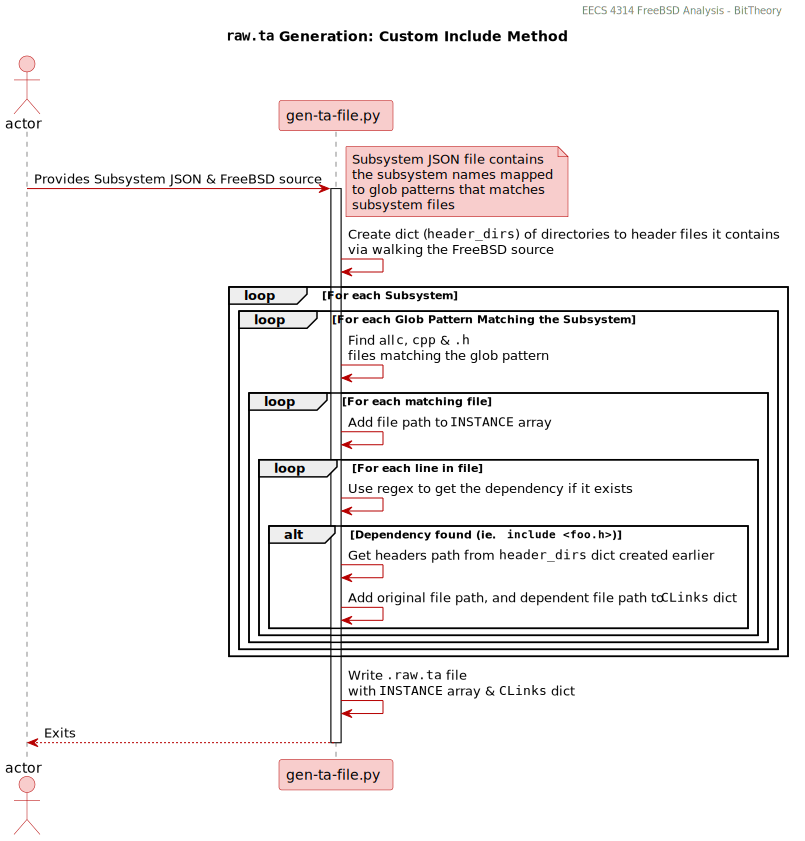
\includegraphics[width = 350pt]{assets/sequence_diagrams/custom_includes.pdf}
	\caption{Raw TA file generation using custom includes script.}
\end{figure}

\begin{figure}[!htb]
	\center
	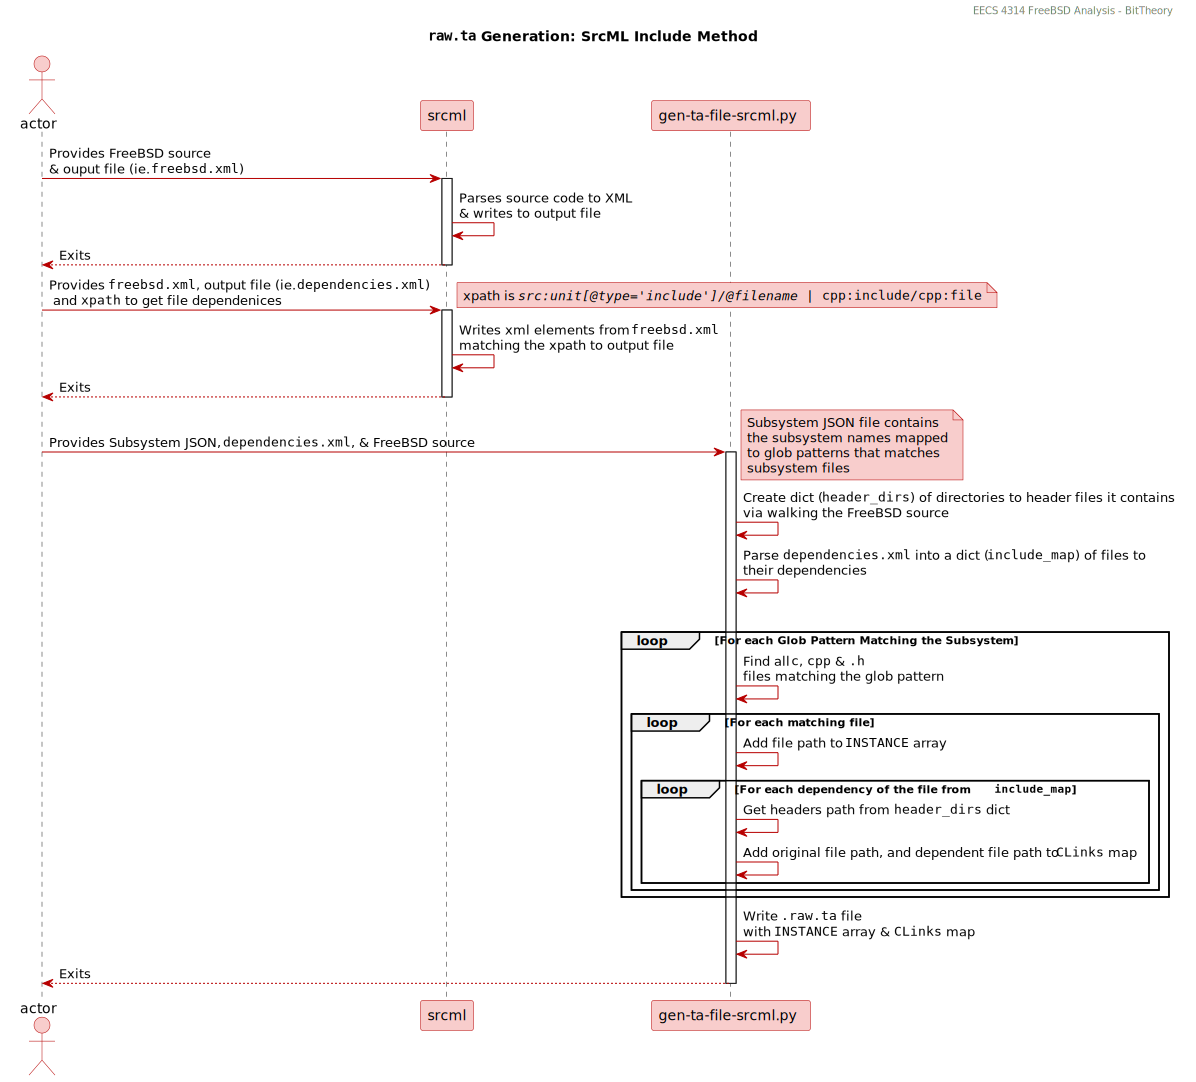
\includegraphics[width = 450pt]{assets/sequence_diagrams/srcml_includes.pdf}
	\caption{Raw TA file generation using custom SrcML script.}
\end{figure}

\section{Quantitative Analysis}
\lipsum[1]

\section{Qualitative Comparison}
\subsection{Process of Qualitative Comparison}
\begin{figure}[h]
    \center
    \includegraphics[width=300pt]{assets/qualitative_process_diagram.PNG}
    \caption{Qualitative Comparison's Process Diagram}
\end{figure}
This is the process of our qualitative comparison. After obtaining the extracted dependencies from each technique, we applied the Stratified Sampling to get samples. Here, the population is the union set of all the techniques minus the common dependencies, which is equivalent to 205,963.
By utilizing a calculator from Creative Research Systems \cite{calculator}, we got 383 as a needed sample size. We divided all the dependencies into 7 stratas and fetched the appropriate number of dependencies from them.
For example, the number of dependencies extracted only by our Custom method is 8, and the proportion of the stratum is 8 divided by 205,963, which is approximately 0.000039.
That is, the sample size needed for the particular stratum is 383 multiplied by 0.000039, which is approximately 0.
After completing all the calculations, we obtained 270 samples from dependencies which only Understand extracted and 113 samples from the common dependencies, extracted by both Custom and srcML methods.
Moreover, we fetched a single random dependency from the other stratas to introduce more variety of reasons for the existence of dependencies in each strata.
After the Stratified Sampling, we observed each dependency to find any differences, examined its file code, and updated our extracters when necessary. We repeated these steps until we classified all the dependencies.
\subsection{Results of Qualitative Comparison}
\subsubsection{Comparison Between Understand and Custom}
\underline{Understand-Only Dependencies}
\newline
\newline
Example$\,\colon\,$\texttt{freebsd/sys/fs/nfsclient/nfs\_clsubs.c \\$\,\to\,$ freebsd/sys/fs/nfsclient/nfs.h}
\newline
\newline
This dependency was extracted because this \texttt{nfs\_clsubs.c} file includes \texttt{nfs.h} as an imported file. Only Understand was able to fetch this dependency as our Custom script is built to fetch the first match, which results in capturing \texttt{nfs.h} under \texttt{sontib/tcpdump} folder.

\underline{Custom-Only Dependencies}
\newline
\newline
Example$\,\colon\,$\texttt{freebsd/sys/dev/pms/RefTisa/sallsdk/spc/sahw.c \\$\,\to\,$ freebsd/sys/dev/pms/RefTisa/sallsdk/hda/64k/iopimg.h}
\newline
\newline
The dependency is found here because ioparray within \texttt{iopimg.h} is included and utilized in \texttt{sahw.c}.
However, Understand did not include this dependency as the used location is within a comment line but within the actual run code. Therefore, it was assumed by Understand that it is an unnecessary dependency to extract.

\underline{Common Dependencies Between Understand And Custom}
\newline
\newline
Example$\,\colon\,$\texttt{freebsd/sys/dev/pms/freebsd/driver/ini/src/agtiapi.c \\$\,\to\,$ freebsd/sys/cam/cam\_sim.h}
\newline
\newline
\texttt{cam\_sim.h} is included and utilized in \texttt{agtiapi.c} for creating structs. For this dependency, Understand simply extracted it, and the Custom script also extracted it without any issues as \texttt{cam\_sim.h} with this particular file name can be found only once in the system.

\subsubsection{Comparison Between Understand and srcML}

\subsubsection{Comparison Between Custom and srcML}
\underline{Custom-Only Dependencies}
\newline
\newline
Example$\,\colon\,$\texttt{freebsd/sys/dev/pms/RefTisa/sallsdk/spc/sahw.c \\$\,\to\,$ freebsd/sys/dev/pms/RefTisa/sallsdk/hda/64k/iopimg.h}
\newline
\newline
It is the same dependency as the one, brought up earlier for the comparison between Understand and Custom. As well as Understand, srcML also ignored the dependency as \texttt{iopimg.h} was included within commented-out lines. 

\underline{srcML-Only Dependencies}
\newline
\newline
Example$\,\colon\,$\texttt{artpqi/smartpqi\_event.c \\$\,\to\,$ freebsd/sys/dev/smartpqi/smartpqi\_includes.h}
\newline
\newline
For this srcML-only dependency, this was included only in a srcML extracted list, and the reason for this was due to the missing white space in include reference.

\underline{Common Dependencies Between Custom And srcML}
\newline
\newline
Example$\,\colon\,$\texttt{freebsd/sys/dev/beri/virtio/network/if\_vtbe.c \\$\,\to\,$ freebsd/sys/amd64/include/cpu.h}
\newline
\newline
For this dependency, we were not able to find a clear rationale. Because both Custom and srcML contain this sample, we first assumed that \texttt{if\_vtbe.c} includes \texttt{cpu.h}. However, after examination, we found out that the \texttt{if\_vtbe.c} imports \texttt{cpu.h}, but not in the path shown in the list of extracted dependencies. Instead, the imported \texttt{cpu.h} was under a \texttt{machine} folder. 
Because the file location is still under the \texttt{machine} folder within a XML file we obtained, we assume that the srcML script we created might need to be modified to show the correct path.

\subsubsection{Performance Metrics}
For the Performance metrics, we utilized recall and precision for our Custom and srcML by including Understand as Oracle.
Here, we have two formulas to calculate recall and precision. As well as these formulas, we included a diagram which shows which dependency sets we examined to obtain solutions.

\begin{equation*}
    \begin{split}
    Recall &= \frac{True Positive}{(True Positive + False Negative)}
    \end{split}
\end{equation*}
\newline
\begin{equation*}
    \begin{split}
    Precision &= \frac{True Positive}{(True Positive + False Positive)}
    \end{split}
\end{equation*}

\begin{figure}[h]
    \center
    \includegraphics[width=300pt]{assets/recall_precision_diagram.PNG}
    \caption{Classification Diagram}
\end{figure}

For both Custom and srcML, we obtained the same results shown below$\,\colon\,$
\newline
For recall, we obtained 66 True Positive dependencies and 270 False Negative dependencies. 
\begin{equation*}
    \begin{split}
    Recall &= \frac{66}{(66 + 270)}\\
    &= 0.196428571\dots\\
    &\approx 20\%
    \end{split}
\end{equation*}
For precision, we obtained the same number of True Positive dependencies and 133 False Positive dependencies.
\begin{equation*}
    \begin{split}
    Precision &= \frac{0 + 66}{(66 + 113)}\\
    &= 0.3687150\dots\\
    &\approx 37\%
    \end{split}
\end{equation*}


\section{Architecture}
\lipsum[1]

\section{Diagrams}
\lipsum[1]

\section{External Interfaces}
\lipsum[1]

\section{Data Dictionary}
\begin{itemize}
	\item{Stratified Sampling: A sampling technique which divides the whole dependency set into multiple strata based on their number proportion}
\end{itemize}

\section{Naming Conventions}
\lipsum[1]

\section{Conclusion}
To conclude, based on the results and observations presented, it is clear that the choice of dependency extraction tool can have a significant impact on the number and types of dependencies identified in a codebase. Understand appears to be the most thorough and comprehensive tool, identifying over 180,000 dependencies, 80% of which were exclusive to that tool. However, it is worth noting that this may lead to more false positives or irrelevant dependencies being identified. SRC-ML and the custom script both focused primarily on include files and identified around 96,000 dependencies, with SRC-ML having no exclusive dependencies and the custom script having only 8. The similarity in their statistics suggests that they may have similar strengths and limitations.

The observation that Understand analyses dependencies based on functions calling other functions while SRC-ML and the custom script prioritise ‘include’ files only suggests that the former may be more effective at identifying dynamic or runtime dependencies, while the latter may be more appropriate for identifying static or compile-time dependencies. However, it is important to note that both types of dependencies can be important in understanding the architecture of a codebase.

In terms of choosing a methodology for dependency extraction in FreeBSD, the specific goals and characteristics of the analysis should be taken into account. For example, if the goal is to identify dynamic dependencies, Understand may be the most appropriate tool. If the focus is on static dependencies based on include files, SRC-ML or the custom script may be more effective. However, it is worth noting that no single tool or methodology may be sufficient on its own, and a combination of techniques may be needed for a more comprehensive understanding of the architecture.

Overall, the process of extracting and analysing architectural dependencies in FreeBSD can be complex and may require careful consideration of the specific needs of the analysis. The tools and methodologies used should be chosen based on the specific goals of the analysis and the characteristics of the codebase being analysed. By taking these factors into account and combining multiple techniques as necessary, a more complete understanding of the architecture of FreeBSD can be achieved.

\section{Lessons Learned}
The importance of choosing the right tool: The choice of tool for dependency extraction can have a significant impact on the results and effectiveness of the analysis. It is important to carefully consider the strengths and limitations of each tool and select the one that is most appropriate for the specific goals and characteristics of the analysis.

The importance of understanding the codebase: A thorough understanding of the codebase is crucial for effective dependency extraction and analysis. Without a good understanding of the code structure, it can be difficult to interpret the results and identify relevant dependencies.

The value of combining multiple techniques: While each tool or methodology may have its own strengths and limitations, combining multiple techniques can provide a more comprehensive understanding of the architecture. For example, using both Understand and a custom script may help to identify both dynamic and static dependencies.

The risk of false positives and irrelevant dependencies: Some tools may identify a large number of dependencies, many of which may not be relevant to the specific analysis. It is important to carefully review and validate the results to avoid being misled by false positives or irrelevant dependencies.

The need for ongoing analysis and refinement: As codebases evolve over time, the architecture and dependencies may change as well. Ongoing analysis and refinement of the dependency extraction process is needed to ensure that the results remain accurate and relevant. This may involve updating the tools and techniques used, as well as revisiting the goals and objectives of the analysis.






\begin{thebibliography}{00}
	\bibitem{b2} Clarke, Arthur C. 2001: A Space Odyssey. New York: Roc, 1968. 297.
	\bibitem{calculator} “Sample Size Calculator.” Sample Size Calculator \- Confidence Level, Confidence Interval, Sample Size, Population Size, Relevant Population \- Creative Research Systems, 2012, https://www.surveysystem.com/sscalc.htm. 
\end{thebibliography}
\end{document}
